\chapter{Independent Component Analysis}\label{app:ICA}
This appendix provide the basic theory of independent component analysis (ICA). The theory is necessary if one wants a deeper understanding towards the justification of applying result from ICA as a reference for evaluation of the main algorithm proposed in this thesis.   
The appendix concludes with an algorithm specifying ICA method which is applied in the thesis. Additionally, an verification test is conducted to evaluate the applied ICA method on the synthetic data, cf. \ref{sec:dataset}.   
\section{Independent Component Analysis}
Independent Component Analysis (ICA) is a method which assume statistical independent, in the EEG signal case, between the sources. With this independence it is possible for ICA to separate the scalp mixture $\mathbf{Y}$ into the sources $\mathbf{X}$ and the mixing matrix $\mathbf{A}$.
\\
Through this section the mathematical concepts of Independent Component Analysis (ICA) will be explained and defined.
\\ \\
Lets set up an situations. We have some measurements that has been affect by some surrounding noise or "\textbf{sideløbende}" measurements such as different conversations in a room. The measurements can be described by a vector $\mathbf{y}$ if we look at the one-dimensional case. $\mathbf{y}$ consist of the measurement from the original signal, a vector $\mathbf{x}$ and surrounding measurements, a matrix $\mathbf{A}$. This situation can be described as the linear model
\begin{align*}
\mathbf{y} = \mathbf{Ax} = \sum_{i=1}^n \mathbf{a}_i x_i
\end{align*}
We known the measurements $\mathbf{y}$ but if also knew the mixing parameter in $\mathbf{A}$ then by inverting the linear model we could solve the system and find the original signal. But this is not the case as the mixing matrix also is unknown.
\\
If we used the statistical properties of $\mathbf{x}$ then it would be possible to estimate both the mixing matrix and then the original signal. What ICA do is to assume statistical independence 
\\ \\
Lets define the ICA model which is a generative model meaning that the observed data is generated by a process of mixing components which are latent component. Let $n$ be the observed random variables such that $y_1, \dots, y_n$ are model as a linear combination of the random variables $x_1, \dots, x_n$:
\begin{align*}
y_i &= a_{i1} x_1 + a_{i2} x_2 + \cdots + a_{in} x_n, \quad i = 1, \dots, n \\
\mathbf{y} &= 
\begin{bmatrix}
a_{11} & a_{12} & \cdots & a_{1n} \\
a_{21} & a_{22} & \cdots & a_{2n} \\
\vdots & \vdots & \cdots & \vdots \\
a_{n1} & a_{n2} & \cdots & a_{nn}
\end{bmatrix}
\mathbf{x}
\end{align*}
where $\mathbf{y} = \{ y_i \}_{i \in [1,n]}$ and $\mathbf{x} = \{ x_t \}_{t \in [1,n]}$. Furthermore, $\mathbf{x}$ is statistically mutually independent.

\subsection{Estimation of Independent Components}
Notes:
Estimation with maximization of nongaussianity (see section 7.5 for nonguassianity)


\subsubsection{Kurtosis}
When estimation ICA with maximization of nongaussianity a measure of the nongaussianity is needed. Kurtosis is quantitative measure used for nongaussianity of random variables. Kurtosis of a random variable $y$ is defined as
\begin{align*}
\text{kurt} (y) = \mathbb{E}[y^4] - 3 ( \mathbb{E}[y^2])^2,
\end{align*}
which is he fourth-order cumulant of the random variable $y$. By assume that the random variable $y$ have been normalised such that its variance $\mathbb{E}[y^2] = 1$, the kurtosis is rewritten as
\begin{align*}
\text{kurt} (y) = \mathbb{E}[y^4] - 3.
\end{align*}
Because of this definition the kurtosis of gaussian random variables will then be zero and for nongaussian random variables the kurtosis will almost always be non-zero \cite[p. 171]{ICA}.
\\
By using the absolute value of the kurtosis gaussian random variables are still zero but the nongaussian random variables will be greater than zero. In this case the random variables are called supergaussian.
\\ \\
For ICA the wish is to maximise the nongaussianity and therefore maximise the absolute value of kurtosis. One way to do this is to you a gradient algorithm.
\\ \\
One complication with the use of kurtosis as measure is the used of measured samples as the kurtosis is sensitive to outliers in the measured data set \cite[p. 182]{ICA}. 

Notes:
A measure of nongaussianity for the vector b which estimate 1 IC
Have some outliners so we introduce negentropy

\subsubsection{Negentropy}
Another measure of nongaussianity is the negentropy which based of the differential entropy known from information theory.
\\
The differential entropy $H$ of a random variable $\mathbf{y}$ with density $p_y (\boldsymbol{\theta})$ is defined as
\begin{align*}
H(\mathbf{y}) = - \int p_y (\boldsymbol{\theta}) \log (p_y (\boldsymbol{\theta}) \ d\boldsymbol{\theta}
\end{align*}
Gaussian random variable has a high entropy.


The negentropy is defined as 
\begin{align*}
J(\mathbf{y}) = H(\mathbf{y}_{\text{gaus}}) - H(\mathbf{y}),
\end{align*}
which is also can be seen as a normalised differential entropy. $\mathbf{y}_{\text{gaus}}$ is a gaussian random variable.

\subsubsection{Approximation of Kurtosis and Negentropy}
\begin{algorithm}[H]
\caption{Gradient Algorithm}
\begin{itemize}
\item[1.] Center the observed data $\mathbf{y}$. $\Delta \mathbf{w} \propto \text{sign}(\text{kurt}(\mathbf{w}^T \mathbf{z})) \mathbb{E}[\mathbf{z} (\mathbf{w}^T \mathbf{z})^3 ]$
\item[2.] $\mathbf{w} \leftarrow \frac{\mathbf{w}}{\Vert \mathbf{w} \Vert}$
\end{itemize}
\end{algorithm}

\paragraph{Notes:}
ICA can be used on Gaussian variables as little is done in addition to decorrelate for Gaussian variable

Whiting is useful to be done beore ICA

A drawback of ICA is the system must be $N \leq M$ meaning that there must more sensors than sources which is not the case in this project where we look at low density EEG system, $M \leq N$. Furthermore, ICA need that the sources are stationary which is not the nature of EEG that are very much nonstationary \cite[p. 7-8]{PHD}.
\\
Instead a mixture model of ICA model where we assume that the amount of activation $k$ in $N$ sources are equal to $M$ (sensor). We can used the short time frame of the sources to make them stationary
 

\section{Fixed-Point Algorithm - FastICA}
An advantage of gradient algorithms is the possibility of fast adoption in non-stationary environments due the use of all input, $\textbf{y}$, at once. A disadvantage of the gradient algorithm is the resulting slow convergence, depending on the choice of $\gamma$ for which a bad choice in practise can disable convergence. A fixed-point iteration algorithm to maximise the non-Gaussianity is an alternative that could be used.

Consider the gradient step derived in section \ref{sec:gra_kur}.
In the fixed point iteration the sequence of $\gamma$ is omitted and replaced by a constant. This builds upon the fact that for a stable point of the gradient algorithm the gradient must point in the direction of $\textbf{b}$, hence be equal to $\textbf{b}$. In this case adding the gradient to $\textbf{b}$ does not change the direction and convergence is achieved.   
Letting the gradient given in \eqref{eq:kurt} be equal to $\mathbf{b}$ and  considering the same simplifications again
suggests the new update step as \cite[p. 179]{ICA}
\begin{align*}
\mathbf{b} \gets \mathbb{E}[\mathbf{y}(\textbf{b}^T \textbf{y})^3] - 3 \mathbf{b}.
\end{align*}
After the fixed point iteration $\textbf{b}$ is again divided by its norm to withhold the constraint $\Vert \textbf{b} \Vert = 1$.   
Instead of $\gamma$ the fixed-point algorithm compute $\mathbf{b}$ directly from previous $\mathbf{b}$.

The fixed-point algorithm is referred to as FastICA. The algorithm has shown to converge fast and reliably, when the current and previous $\mathbf{b}$ point in the same direction \cite[p. 179]{ICA}. 

\subsection{Negentropy}
An alternative measure of non-Gaussianity is the negentropy, which is based on the differential entropy. The differential entropy $H$ of a random vector $\mathbf{y}$ with density $p_y (\boldsymbol{\eta})$ is defined as
\begin{align*}
H(\mathbf{y}) = - \int p_y (\boldsymbol{\eta}) \log (p_y (\boldsymbol{\eta})) \ d\boldsymbol{\eta}.
\end{align*}
The entropy describes the information that a random variable gives. The more unpredictable and unstructured a random variable is higher is the entropy, e.g. Gaussian random variables have a high entropy, in fact they have the highest entropy among the random variables of the same variance \cite[p. 182]{ICA}.

Negentropy is a normalised version of the differential entropy such that the measure of non-Gaussianity is zero when the random variable is Gaussian and non-negative otherwise. The negentropy $J$ of a random vector $\mathbf{y}$ is defined as 
\begin{align*}
J(\mathbf{y}) = H(\mathbf{y}_{\text{gauss}}) - H(\mathbf{y}),
\end{align*}
with $\mathbf{y}_{\text{gauss}}$ being a Gaussian random variable of the same covariance and correlation as $\mathbf{y}$ \cite[p. 182]{ICA}.
As the kurtosis is sensitive for outliers, the negentropy is instead difficult to compute computationally as the negentropy require a estimate of the pdf. As such an approximation of the negentropy is needed.
To approximate the negentropy it is common to use the higher order comulants including the kurtosis. The following approximation of the scalar case is stated without further elaboration, the derivation can be found in \cite[p. 183]{ICA}. 
\begin{align*}
J(\mathbf{y}) \approx \frac{1}{12} \mathbb{E}[y^{3}]^2 \frac{1}{48}\text{kurt}(y)^2.
\end{align*}


\subsection{Fixed-Point Algorithm with Negentropy}
Maximization of negentropy by use of the fixed-point algorithm is now presented, for derivation of the fixed point iteration see \cite[p. 188]{ICA}. Algorithm \ref{alg:fastICA} show Fast ICA using negentropy, this is the algorithm which is applied in the thesis for comparison with the source recovery methods which are tested in this thesis.    

\begin{algorithm}[H]
\caption{Fast ICA -- with negentropy }
\begin{algorithmic}[1]
			\Procedure{Pre-processing}{$\textbf{y}$}
			\State $\text{Center measurements} \quad \textbf{y} \gets \textbf{y} - \bar{\textbf{y}}$
			\State $\text{Whitening} \quad \textbf{y}\gets \textbf{y}_{white}$ 
			\EndProcedure  
			\State
            \Procedure{FastICA}{$\textbf{y}$}    
			\State$k=0$            
            \State$\text{Initialise random vector} \quad \textbf{b}_{(k)}$ \Comment{unit norm}
            \For{$j \gets 1,2, \hdots ,N$ }
            
            	\While{$\text{convergance critia not meet}$} 
               		\State $k = k+1$
                	\State $\textbf{b}_{(k)} \gets \mathbb{E}[ \textbf{y}(\textbf{b}_{(k-1)}^T \textbf{y})] - \mathbb{E}[g'(\textbf{b}_{(k-1)}^T \textbf{y})] \textbf{b}_{(k-1)}$ \Comment{$g$ cf. \cite[p. 190]{ICA}} 
                	\State $\textbf{b}_{(k)} \gets \textbf{b}_{(k-1)}/\Vert \textbf{b}_{(k-1)} \Vert $ 
          		\EndWhile
          		\State $x_{j} = \textbf{b}^T\textbf{y}$
          	\EndFor
          	
            \EndProcedure
        \end{algorithmic} 
        \label{alg:fastICA}
\end{algorithm}


\section{Verification of fast ICA on synthetic data}\label{app:ica_test}
The purpose of this section is to verify the fast ICA algorithm which is used in this thesis. By this verification the purpose is to justify the ICA algorithm as a reference point with respect to performance of the developed main algorithm.

The fast ICA algorithm is tested on synthetic data simulated as described in section \ref{sec:dataset}. 
Consider the following linear system, which makes a model of EEG measurements.  
\begin{align*}
\textbf{Y}=\textbf{AX}
\end{align*}
where $\textbf{Y}^{M\times L}$, $\textbf{A}^{M\times N}$ and $\textbf{X}^{N\times L}$. It is expected that the fast ICA algorithm manage to solve the linear system for $\textbf{X}$ and $\textbf{A}$ given only the measurements $\textbf{Y}$, in the case where $M=N$.  

The fast ICA algorithm is applied to $\textbf{Y}$ and returns the estimates $\hat{\textbf{X}}_{ICA}$ and $\hat{\textbf{A}}_{ICA}$. 
When using the fast ICA algorithm the output $\hat{\textbf{X}}_{ICA}$ do not correspond one to one with the true source signal, which become an issue when the estimation error is measured by the mean squared error (MSE) cf. subsection \ref{sec:mse}.  The fast ICA algorithm is invariant towards the amplitude and phase of the signal and furthermore the rows are not necessarily place the original location. 
In order to get a valid MSE measure of the estimate, a function is defined to fit the estimate to the true source signal $\textbf{X}$. The function manage to pair the rows and change the phase, such that the total MSE is minimized. Furthermore each row of the estimate is scaled by the relationship between the maximum value of the true row and the estimated row.
From empirical observations only the phase shift performed by multiplying with $(-1)$ has shown necessary, hence it is easily applied to the fitting function.
When the fitting function is applied two the estimate, the full potential of the fast ICA algorithm is considered reached.       

Figure \ref{fig:appica1} illustrates $\hat{\textbf{X}}_{ICA}$, without use of the fitting function, resulting from the fast ICA algorithm applied to a simulated deterministic data set $\textbf{Y}$ specified by $M=N=k=4$ and $L=1000$. In the figure $\textbf{Y}$, $\textbf{X}$ and $\hat{\textbf{X}}_{ICA}$ are plotted separately and it is clear to see the invariance towards amplitude and phase.
The MSE from the original $\hat{\textbf{X}}_{ICA}$ becomes
\begin{align*}
MSE(\textbf{X},\hat{\textbf{X}}_{ICA}) = 0.608.
\end{align*}

In figure \ref{fig:appica2} the fitting function has been applied to $\hat{\textbf{X}}_{ICA}$. Each row of the fitted estimate is now plotted with the corresponding row of the true source signals. 
The resulting MSE becomes 
\begin{align*}
MSE(\textbf{X},\hat{\textbf{X}}_{ICA}) = 0.046.
\end{align*}  
This is an essential change from the first measured MSE, and it is considered to provide a more valid measure of the estimate. From the visualisation and the corresponding MSE it is found that the fast ICA algorithm manage to estimate the source signals of the deterministic data set with a sufficiently small error. 
\begin{figure}[H]
    \begin{minipage}[t]{.45\textwidth}
		\centering
		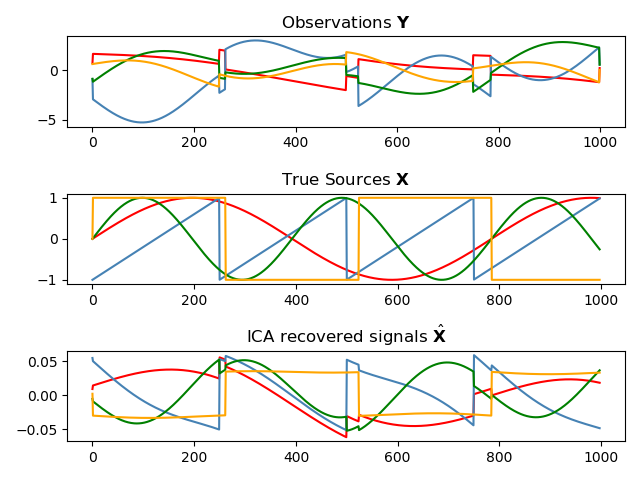
\includegraphics[scale=0.45]{figures/ICAapp/ICA_app1.png}
	\caption{Plot of simulated deterministic observations $Y$, specified by $M=N=k=4$ and $L=1000$. Corresponding plot of the true $\textbf{X}$ and the estimated $\hat{\textbf{X}}$ by ICA.}
	\label{fig:appica1}
    \end{minipage} 
    \hfill
    \begin{minipage}[t]{.45\textwidth}
		\centering
		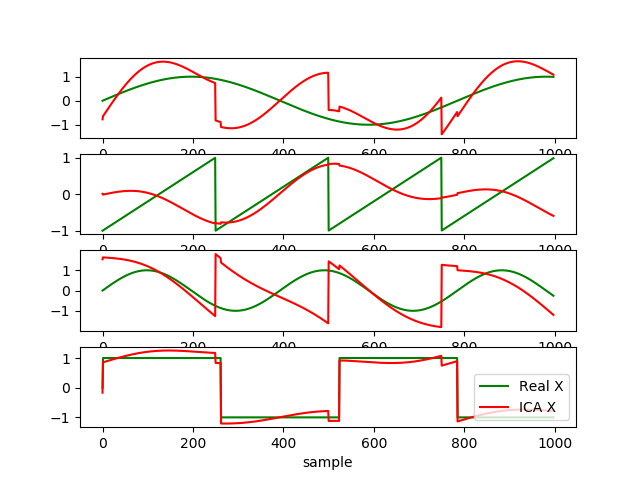
\includegraphics[scale=0.45]{figures/ICAapp/ICA_app2.png}
	\caption{Direct comparison of the true $\textbf{X}$ and $\hat{\textbf{X}}_{ICA}$ after applying the fitting function.}
	\label{fig:appica2}
    \end{minipage}
\end{figure}

A similar test is now performed on a stochastic data set  $\textbf{Y}$, cf. section \ref{sec:stoch_data}, again specified by $M=N=k=4$ and $L=1000$. 
Figure \ref{fig:appica3} show the comparison of the fitted $\hat{\textbf{X}}_{ICA}$ and the true source signals $\textbf{X}$. Note that only the first 100 samples are plotted for easier visualization. The resulting MSE becomes:
\begin{align*}
MSE(\textbf{X},\hat{\textbf{X}}_{ICA}) = 0.037.
\end{align*}       
Again the the MSE is considered sufficiently small and by that the fast ICA is considered verified with respect to solving a linear system with $M=N$. 
\begin{figure}[H]
	\centering
	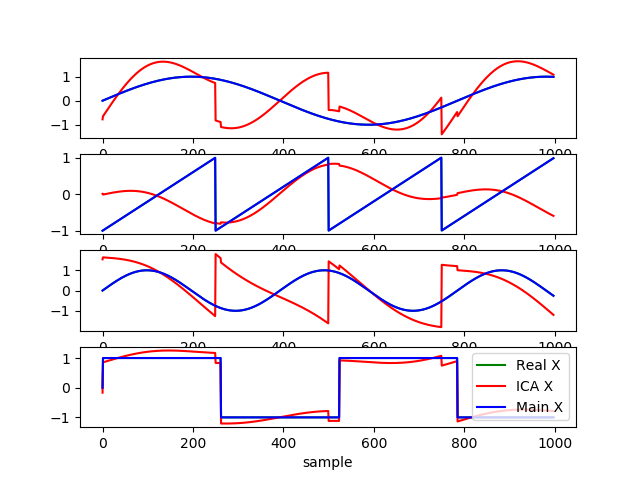
\includegraphics[scale=0.5]{figures/ICAapp/ICA_app3.png}
	\caption{ICA applied to stochastic simulated observations $\textbf{Y}$. Direct comparison of the true $\textbf{X}$ and $\hat{\textbf{X}}_{ICA}$ after applying the fitting function.}
	\label{fig:appica3}
\end{figure}

Consider now the case where $k \leq N=M$, that is the sources signal matrix has $k$ non-zeros rows. 
The fast ICA algorithm is now applied to a stochastic data set $\textbf{Y} $ specified by $N=M=6$, $k = 4$ and $L=1000$. Figure \ref{fig:appica5} and \ref{fig:appica6} show the comparison of the resulting $\hat{\textbf{X}}_{ICA}$ and the true $\textbf{X}$ before and after the application of the fitting function, respectively. The resulting MSE becomes:
\begin{align*}
MSE(\textbf{X},\hat{\textbf{X}}_{ICA}) = 1.784.
\end{align*} 
It is seen from figure \ref{fig:appica6} that the fast ICA algorithm manage to  detect the zero rows of $\textbf{X}$. Without further test, this indicates the possibility of estimating $k$ from the fast ICA algorithm. 
\begin{figure}[H]
    \begin{minipage}[t]{.45\textwidth}
		\centering
		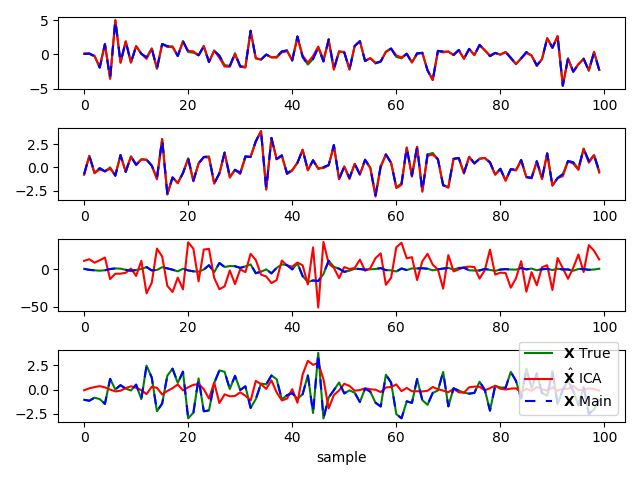
\includegraphics[scale=0.5]{figures/ICAapp/ICA_app5.png}
	\caption{}
	\label{fig:appica5}
    \end{minipage} 
    \hfill
    \begin{minipage}[t]{.45\textwidth}
		\centering
		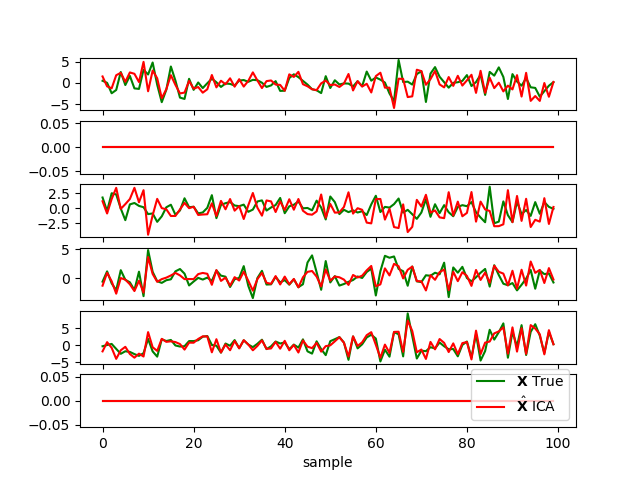
\includegraphics[scale=0.5]{figures/ICAapp/ICA_app6.png}
	\caption{}
	\label{fig:appica6}
    \end{minipage}
\end{figure}

With these tests the quality of the fast ICA algorithm has been verified. As such the fast ICA algorithm can be used as a reference, when applied to real EEG data. It is further established that $k\leq M$ can be estimated by fast ICA. 

Remember though that the ICA estimate is conditioned under $k\leq N=M$, however this condition is not necessarily withhold for real EEG measurements as the true $N$ is always unknown.   











  


